\chapter[Introdução, \emph{por Caio Gagliardi}]{Introdução}
\hedramarkboth{Introdução}{Caio Gagliardi}

\textsc{Fernando Pessoa} planejou uma grande obra teatral, antes concebida para
ser lida do que encenada. Embora tenha escrito mais de trinta peças em
português e em inglês, em prosa e em verso, a sua quase totalidade foi
deixada inacabada e desconhecida do grande público. Em algumas
anotações do autor a respeito dessa fração menos conhecida de sua obra,
encontramos registrada a expressão “Teatro d’êxtase”, que emprestamos a
esta edição. 

Não há uma listagem completa das peças que comporiam esse conjunto, mas é certo
que a palavra “êxtase” identifica uma característica comum às que aqui
estão reunidas: nelas, há sempre um momento em que as personagens
parecem encarnar a figura do sonhador visionário, que viaja, através de
conjecturas, para além do real imediato, deixando-se absorver por um
estado de consciência independente de toda e qualquer ação externa. O
substantivo “êxtase” (do grego \textit{ekstasis}) refere-se a um estado
da alma absorta na contemplação de Deus e do mundo sobrenatural,
definição que condiz, de modo mais ou menos direto, com os enredos das
peças, em que há sempre uma forma de intuição ou vidência que é
atribuída a uma de suas personagens. Ainda do ponto de vista
psicanalítico --- que não era estranho a Pessoa ---, “êxtase” é um estado
nervoso caracterizado pela perda da consciência da própria existência,
o que sintetiza bem, como veremos mais adiante, um dos momentos de
\textit{O marinheiro}, a principal peça que integra este conjunto.

\section{\mbox{Das peças que integram esta edição}}

\textit{O marinheiro} foi a única peça publicada em vida por Pessoa. Foi
com ela, aliás, que seu autor, até então mais conhecido pelo leitor
português como polemista e crítico literário, estreou no primeiro
número da revista \textit{Orpheu}, a publicação mais importante do
modernismo em Portugal. Segundo Pessoa, a peça teve uma primeira versão em 1913
(conforme a data que acrescenta ao seu final), e foi revisada até a sua
publicação, em 1915. Além disso, \textit{O marinheiro} antecipa com
especial habilidade artística aspectos marcantes da poética pessoana,
dentre os quais o processo de despersonalização dramática, da qual
resulta a heteronímia. Devido à sua importância central para o conjunto
da obra de Fernando Pessoa --- embora não fosse demasiado afirmar, para a
história do teatro em língua portuguesa ---, optamos por dedicar-lhe um
estudo exclusivo. 
\renewcommand{\caption}[1]{{\small\textit{#1}}}
\begin{figure}
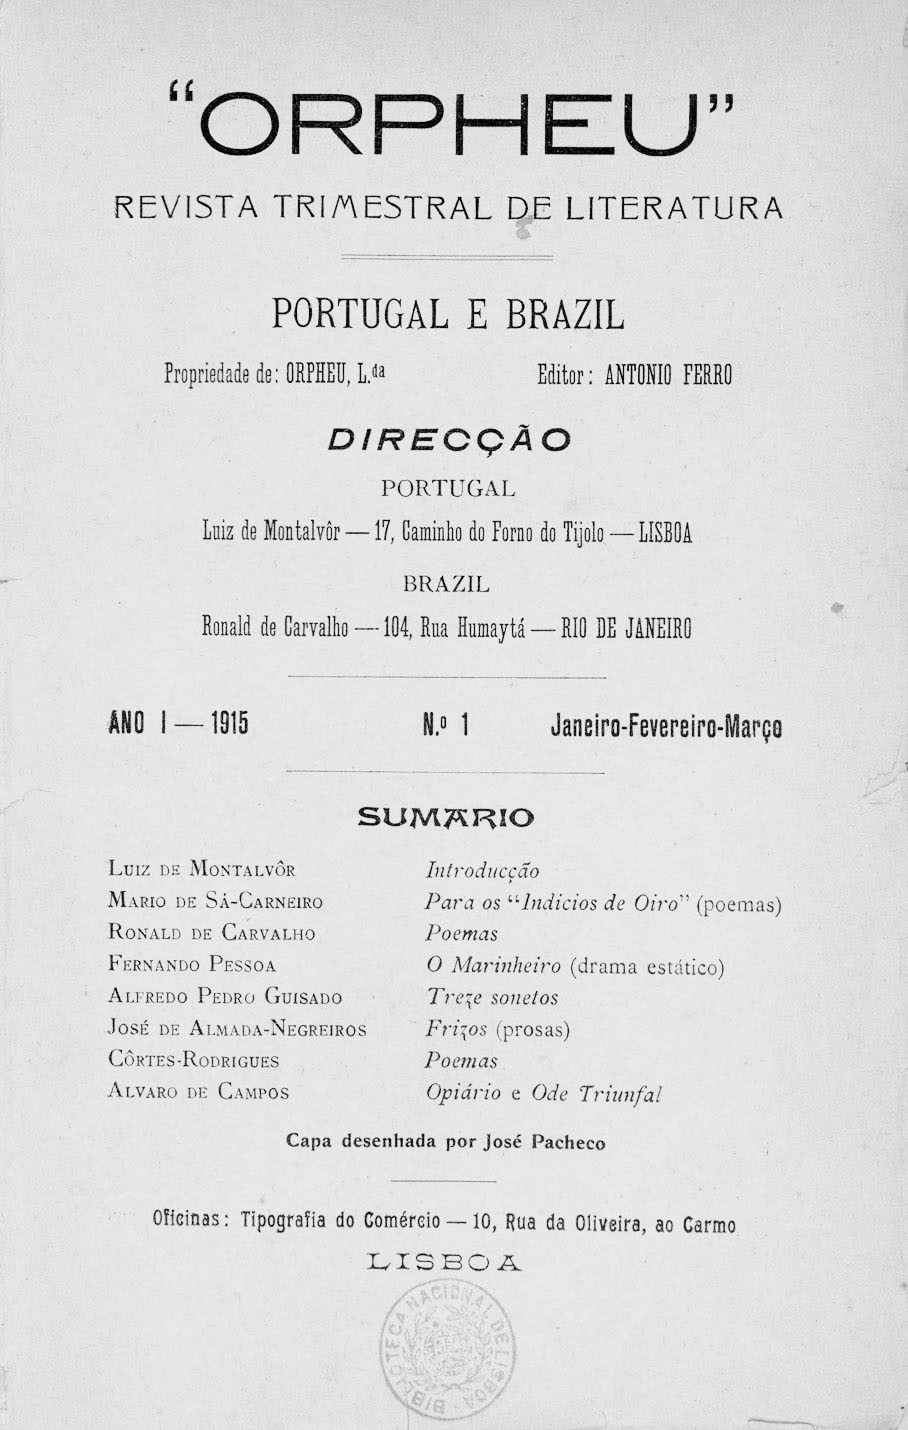
\includegraphics[width=\textwidth]{3.png}
\caption{Frontspício do n.~1 da revista \emph{Orpheu}}
\end{figure}

Além de \textit{O marinheiro}, reúnem-se aqui outros quatro dramas,
\textit{A morte do príncipe}, \textit{Diálogo no jardim do
palácio}, \textit{Salomé} e \textit{Sakyamuni}.\footnote{ Esses textos
são, na sua origem, manuscritos e fragmentos datilografados encontrados em folhas dispersas,
incluindo alguns exemplares da revista \textit{A águia}. 
Muitas dessas páginas não foram identificadas pelo autor, e, à margem do texto, 
Pessoa deixou anotadas variantes para muitos termos que empregou, o que revela seu estágio ainda
inacabado.
Todo esse material foi transcrito, coligido e ordenado pela
crítica portuguesa Teresa Rita Lopes, sem a qual a expressão “o teatro
de Pessoa” teria uma dimensão bem mais restrita do que a atual. Com
exceção ao \textit{Fausto}, texto escrito durante toda a vida literária
de seu autor, as peças aqui publicadas são aquelas que apresentam
melhor acabamento formal.}

\textit{A morte do príncipe} recebeu encenações em Portugal e na
Argentina, e foi adaptada para o cinema em 1991, com o mesmo título e
sob direção de Maria de Medeiros. Trata-se de um texto praticamente
acabado, que remete aos monólogos de \textit{Hamlet}, de Shakespeare,
mas com fortes ecos de Mallarmé: “Todo este universo é um livro em que
cada um de nós é uma frase”. Difícil não projetar sobre a personagem
“X” a figura de Horácio, fiel amigo de Hamlet. O tom de certas
passagens de teor metalinguístico é o mesmo atingido por trechos
análogos do \textit{Livro do desassossego}. A exemplo das demais
personagens das peças aqui reunidas, o príncipe alcança, através de sua
viagem delirante pelos arcanos da própria alma, uma espécie de êxtase
visionário, de crise perceptiva, que o leva a afirmar que a única
realidade reside no sonho, isto é, não na própria vida, mas no teatro
da vida: “As princesas que eu sonhei é que existem\ldots{} As da terra são
apenas as bonecas com que as outras brincam, vestindo-as, corpo e alma,
a seu modo\ldots{}”
Entre os fragmentos que foram reunidos para recompor a peça, duas páginas foram
datilografadas no verso de um panfleto em defesa de Raul Leal, atacado por uma organização 
de estudantes, ``Sobre um Manifesto de Estudantes'', escrito em 
abril de 1923. Além disso, Teresa Rita Lopes transcreveu uma folha datilografada
que traz a data de 05--10--1932.
Embora dialogada, toda a cena se passa como se fosse um
monólogo.

\textit{Diálogo no jardim do palácio} é também uma peça aparentemente
concluída, que guarda fortes ecos dos diálogos platônicos,
especificamente no que tange a reflexão sobre o amor e a dicotomia
entre corpo e alma. Como acontece com as demais peças aqui publicadas,
este diálogo entre duas personagens, apenas indicadas por A e B, é um
interlúdio temporal, uma espécie de suspensão cronológica em que o eu
se observa cindido em dois, refletindo sobre a tópica do \textit{amabam
amare} (amar o amor), de Santo Agostinho, e antecipando a reflexão mais
sistemática que Pessoa realizaria no âmbito “sensacionista”: 
\begin{hedraquote}
Há grandes interiores de continentes dentro de nós, com mistérios a
desvendar. Quem sabe, amor, se raças diferentes das nossas habitarão
esses sítios desconhecidos (inexplorados)? Habituei-me sempre a olhar
para as minhas sensações como para uma coisa exterior.
\end{hedraquote}

Parte do texto
foi escrita à mão em algumas páginas de um dos números da revista
\textit{A águia}, de 1913. Este diálogo foi representado em conjunto
com as outras peças aqui mencionadas, em Portugal e no Brasil.
\begin{figure}
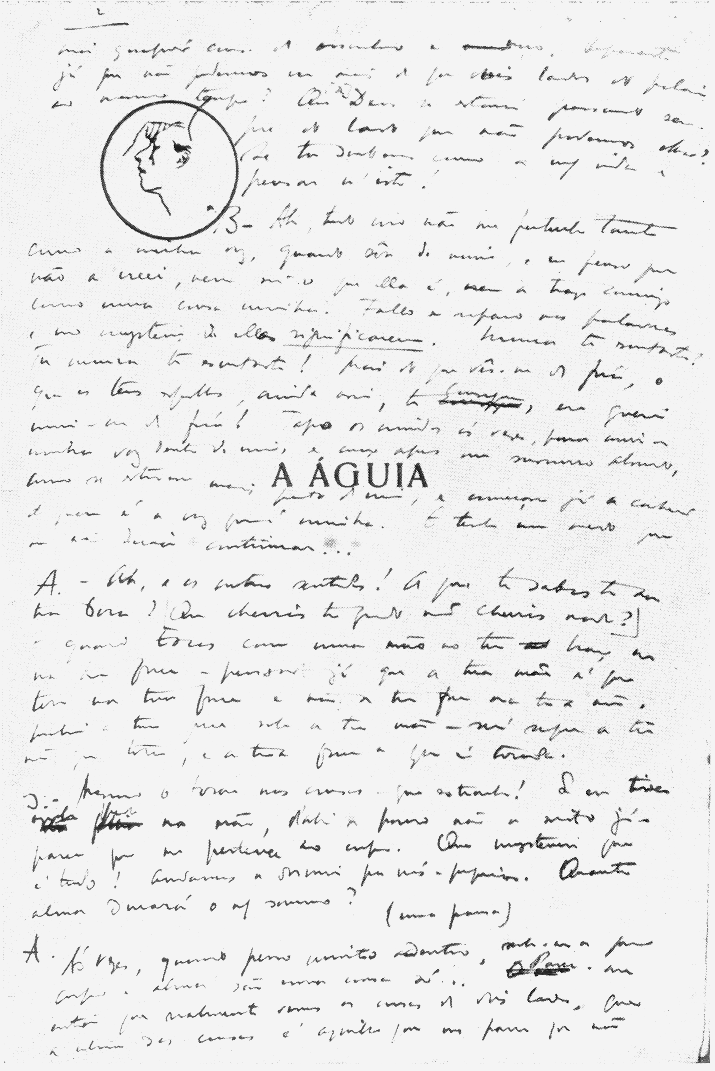
\includegraphics[width=\textwidth]{4.png}
\caption{Manuscrito feito sobre a edição da revista \emph{A águia}}
\end{figure}

Com \textit{Salomé}, Pessoa insere-se na rica tradição de releituras do
tema bíblico da \textit{mulher fatal}, que povoa o imaginário cultural
dos finais do século \textsc{xix}. Apontada como executora de João Batista, no
\textit{Novo Testamento}, Salomé foi retratada na pintura de Moreau, na
ópera de Strauss e na literatura de autores como Flaubert, Mallarmé,
Wilde, Huysmans e Laforgue. A peça que Fernando Pessoa nos legou, e na
qual alcança inaudita suspensão onírica, é uma das menos conhecidas
entre as releituras que o mito bíblico inspirou. Embora fragmentada, a
\textit{Salomé} de Pessoa já ganhou os palcos, além de ter se
transformado em ópera de câmara em seu país de
origem. Uma das páginas desse drama foi manuscrita no verso de uma carta
datada de 9 de março de 1914.

Finalmente, \textit{Sakyamuni} é uma
espécie de encenação budista que pertenceria a um conjunto de três
peças, das quais conhecemos somente um outro título, \textit{Calvário},
esta centrada na figura de Cristo. \textit{Sakyamuni} retoma o processo
de ascensão do príncipe do Himalaia, Siddhartha Gautama (566--468 a.C.),
a Sakyamuni, ou seja, o sábio do clã Shakya, e posteriormente sua
iluminação, a partir da qual passou a ser chamado de Buda. O termo
\textit{Boddhisattva} era usado pelo Buda para se referir a si mesmo em
todo o período anterior à sua iluminação, incluindo suas vidas
anteriores. “Buda” foi, inclusive, um título cogitado por Pessoa para
esse drama. Sem indicação de data, a peça nos sugere interessante clave de leitura para o
vertiginoso processo de despersonalização poética em que resultou a
heteronímia: “Tornado a Diversidade Absoluta, o Abismo Puro, morrerás
de ti próprio. E tudo será o Nirvana atingido, e o Fim [dourado] da
Estrada''.


\section{O espaço primordial do\break drama em \textls{O marinheiro}}

Pessoa definiu \textit{O marinheiro} como um
\textit{drama estático}. A expressão, em voga entre
autores franceses do fim do século \textsc{xix}, revela
a existência de uma forte identidade entre sua peça e o teatro
simbolista dos anos 1890, no qual, amiúde, os diálogos 
não são senão intervalos que preparam o leitor para 
as pausas e os longos silêncios,
e em que a encenação apresenta forte apelo simbólico.
Assim como sucedeu com o romance, o teatro simbolista 
foi responsável por superar
as convenções naturalistas de representação. Não se tratava, ao
contrário do que se pode pensar, de uma experiência 
de ruptura, pura e simplesmente; o ``\textit{théatre statique}'',
tal como referido por seus epígonos
de língua francesa, antes de designar um gênero, teria sido uma
qualidade própria das grandes peças da Antiguidade Clássica. Para o
principal nome do teatro desse período, 
o belga Maurice Maeterlinck, a
maior parte das tragédias de Ésquilo são 
``\textit{tragédies immobiles}''. Mas o
protótipo desse tipo de drama é 
\textit{Hamlet}, de Shakespeare. A seu
respeito, não é impreciso afirmar que os 
monólogos interiores de seu
protagonista provocaram verdadeiro fascínio no imaginário
simbolista.\footnote{ M. Maeterlinck.
\textit{Le Trésor des Humbles}.
Apud Teresa Rita Lopes. \textit{Fernando Pessoa 
et le drame simboliste: héritage et création}.
Lisboa, Paris, Foudation Calouste Gulbenkian:
Centre Culturel Portugais, 1985, p.~17.} Em síntese, o drama
simbolista conferiu à \textit{imobilidade} o status
de valor próprio das grandes peças. 

Segundo Robert Bréchon, com o seu drama \textit{Os cegos} (1890),
Maeterlinck forneceu a \textit{O marinheiro} seu 
“modelo formal da ação dramática”.\footnote{ Robert Bréchon.
\textit{Estranho estrangeiro}.
Rio de Janeiro: Record, 2000. pp.~176--7.} 
Teresa Rita Lopes, autora do
mais importante trabalho sobre a relação de Pessoa com o drama
simbolista, revela que a biblioteca do poeta, hoje 
hospedada na Casa Fernando Pessoa, em Lisboa, 
contém a mais conhecida peça de Maeterlinck,
\textit{Les Aveugles}, profusamente anotada. Para
a pesquisadora, a identificação de influências não deve sugerir,
contudo, uma relação de dívida com o teatro simbolista, uma vez que
\textit{O marinheiro} supera, enquanto realização formal e 
em densidade psicológica, seus modelos imediatos.

Outra característica que o drama simbolista emprestou a \textit{O
marinheiro} é a sublevação das personagens com relação às suas
falas. Em outras palavras, no drama simbolista as personagens 
parecem sempre menos importantes do que as palavras que enunciam. 
Elas, por vezes, chegam mesmo a se espantar com o que dizem. 
Esse traço é marcante em autores como Mallarmé e Hofmannsthal, 
que, nas palavras de Anna Balakian, cultivaram o “poder mágico 
da palavra”.\footnote{ Anna Balakian.
\textit{O simbolismo}. São Paulo: 
Perspectiva, 1985, p.~109.} O que talvez seja axial 
nessa concepção de teatro é sua aproximação com a
poesia, gênero em que as palavras apresentam especial densidade.
Algumas peças de Yeats, por exemplo, são derivações de seus 
poemas, o que é um dado representativo da ausência de 
fronteiras bem demarcadas entre os gêneros.
Afinal, tratava"-se já de um teatro lírico de ruptura
com as convenções do drama, cujo tom sepulcral delegava
à morte seu papel simbólico central. 

Num manuscrito, provavelmente de 1914, Pessoa formula
essa sua concepção de teatro:

\begin{hedraquote}
Chamo teatro estático àquele cujo enredo 
dramático não constitui ação ---
isto é, onde as figuras não só não
agem, porque nem se deslocam nem
dialogam sobre deslocarem"-se, mas
nem sequer têm sentidos capazes de
produzir uma ação; onde não há conflito
nem perfeito enredo. Dir"-se"-á
que isto não é teatro. Creio que o é
porque creio que o teatro tende a
teatro meramente lírico e que o enredo
do teatro é, não a ação nem a
progressão e consequência da ação ---
mas, mais abrangentemente, a
revelação das almas através das 
palavras trocadas e a criação de
situações [\ldots{}]. Pode haver revelação
de almas sem ação, e pode haver
criação de situações de inércia, momentos 
de alma sem janelas ou portas
para a realidade.\footnote{ Fernando Pessoa. \textit{Páginas de estética e de teoria e crítica
literárias}. 2ª. ed., org.~de Georg Rudolf Lind e Jacinto do Prado
Coelho. Lisboa: Ática, 1973, p.~112.}
\end{hedraquote}

O quarto, onde transcorre \textit{O marinheiro}, tem o formato circular, a exemplo do palco grego,
cujo centro, destinado ao plano terrestre da representação,
é também esférico. No centro do quarto, por sua vez, no alto
de uma mesa, há um caixão onde jaz uma donzela de branco.
Não sabemos quem ela foi, que relação teve
com suas veladoras, tampouco quando e em que lugar se situa esse
castelo. A indicação isolada de que ele
é \textit{antigo} se apresenta
como indício de uma ancestralidade mítica, isto é, de que a cena se
passe fora do tempo histórico. Estamos diante de um 
drama imemorial,
portanto, cujo prenúncio já se revela em sua primeira 
fala, “Ainda não
deu hora nenhuma”, e perpassa todo o texto, “Quem sabe se nós
poderíamos falar assim se soubéssemos a hora que é?”.
A vigília das três
donzelas --- não por acaso identificadas como “veladoras” ---
assume já um caráter alegórico no drama, por atuar como 
metáfora da existência. Daí
a ancestralidade que é própria, afinal, do
\textit{leitmotiv}, do seu motivo condutor:
a morte ocupa o centro do quarto e do drama, e as
veladoras, à sua volta, como Sherazade para escapar a ela,
conversam,
contam histórias, suspendendo a \textit{physis},
a realidade ou seu fim natural. 
Exemplar é, por isso, a fala da segunda veladora: “Contemos
contos umas às outras\ldots{} Eu não sei contos nenhuns, 
mas isso não faz mal\ldots{} Só viver é que faz mal\ldots{}”. 
``Navegar é preciso, viver não é
preciso'', afirmará Pessoa mais tarde. Eis um dos 
frutos semeados por \textit{O marinheiro} em sua poética.

Curiosamente, esse caráter \textit{mítico} da peça não impede, ao
contrário do que se poderá supor, que ela respeite a lição 
aristotélica da unidade de espaço e de tempo: 
o drama pessoano apresenta tanto
duração definida --- transcorre no período de
uma madrugada --- quanto, como se disse, espaço
demarcado --- a torre de um castelo. Além disso,
chama a atenção o fato de a tragédia antiga 
nunca apresentar mais do
que três personagens contracenando, exatamente 
o número de donzelas em
\textit{O marinheiro}. Os tragediógrafos antigos 
observavam a regra de
não falar uma quarta personagem numa mesma cena, conforme vem
registrado no preceito de Horácio, na epístola aos Pisões,
``\textit{nec quarta loqui persona laboret}'' literalmente 
``e uma quarta personagem não se empenhe em
falar''.\footnote{ Horácio. \textit{Arte poética}. Ed.
bilíngue. Trad.  R. M. Rosado Fernandes. Lisboa: Clássica, s.~d.
v.~193.} No \textit{Agamêmnon},
de Sêneca, por exemplo, no último ato,
Cassandra, embora o tempo todo presente em cena, junto com
Clitemnestra, Egisto e Electra, só fala depois que esta última se
retira, levada para o exílio.\footnote{ Sêneca,
\textit{Agamêmnon}.
Intro., trad. e org. de José Eduardo Lohner.
São Paulo: Globo,
2009.} Em \textit{O marinheiro}, a quarta personagem está morta. 

Ao que parece, existe nesse drama um jogo de definições e
indefinições que não pode ser desprezado.

Embora tenha sido produzido em prosa, \textit{O marinheiro} é 
permeado
de um lirismo sugestivo, cinzelado por pausas e reticências.
Associado
a ele, a sensação de irrealidade acompanha sua leitura, como se uma
leve bruma encobrisse a cena única, toldando"-a com uma atmosfera de
sonho, própria da sondagem psicológica presente nos diálogos. Essa
atmosfera carrega também algo de sinistro. Isso porque a 
condução do
drama é análoga à de um suspense metafísico: em mais de um momento das
falas das personagens, algo parece estar para ser revelado, e a
previsão dessa descoberta causa"-lhes espanto e temor. 

Vem a propósito desse comentário um importante trecho escrito em inglês
por Pessoa, traduzido pelo crítico José Augusto Seabra, no qual o
escritor sublinha o caráter trágico da peça e revela seu juízo
especialmente positivo sobre o desenlace:

\begin{hedraquote}
Começando de uma forma muito simples, o drama evolui 
gradualmente para
um cume terrível de terror e de dúvida, 
até que estes absorvem em si as
três almas que falam e a atmosfera da 
sala e a verdadeira potência do
dia que está para nascer. O fim da peça 
contém o mais sutil terror
intelectual jamais visto. Uma cortina de 
chumbo tomba quando elas não
têm mais nada a dizer uma às outras nem mais nenhuma razão para
falar.\footnote{ Apud José Augusto Seabra.
\textit{Fernando Pessoa ou
o poetodrama}. São Paulo: Perspectiva, 1974, p.~31. O trecho vem
reproduzido no original segundo a edição da \textit{Obra poética} 
da Nova Aguilar.}
\end{hedraquote}

A ausência de demarcação do tempo histórico
da cena está associada à
sensação de irrealidade que ela produz em seu leitor e nas próprias
personagens. Estas, por seu turno, não compõem 
um conflito; ao invés de
agirem, apenas conversam, e seus diálogos são 
prolíficos em conjecturas
existenciais. As falas das veladoras, a certa 
altura da peça, deixam de
demarcar espaços de enunciação distintos ou de identificar as
personagens, para confundi"-las umas com as outras. Ganha força a
sensação no leitor de que essas vozes não se prendem a um corpo
definido. À medida que a leitura avança, as veladoras se evanescem,
desmaterializam"-se enquanto personagens, e as falas, 
já incorpóreas, e
sem referência no espaço e no tempo, deixam transparecer o tom
monocórdio do texto. O diálogo se enfraquece a ponto de 
se remodular em
uníssono, e as três vozes convergem, finalmente, 
num monólogo. A partir
de então, a leitura já não é a de um drama que se 
passa na torre de um
castelo, mas dentro da mente humana. Das veladoras, embora ainda
identificadas como enunciadoras, resta apenas o espectro, e a peça,
como que nos convidando à releitura, permite entrever sua imagem
latente: de uma única personagem em conversa consigo mesma. Eis o
espaço primordial desse drama.

\paragraph{Uma \textit{plaquette} ou o mais alto grau do sonho}

Em 1915, Fernando Pessoa já havia escrito alguns dos 
seus principais
poemas, incluindo parte importante da poesia 
heteronímica. Dentre um
conjunto notável de textos, Pessoa escolhe
\textit{O marinheiro} para
figurar como seu primeiro texto publicado na
\textit{Orpheu}, a revista
que inaugura o modernismo em Portugal,
e certamente a mais genuinamente
pessoana delas. A \textit{Orpheu} veicula 
também, mais adiante, dois
textos antológicos de Álvaro de Campos, a
“Ode triunfal” e “Opiário”,
embora estes poemas não façam parte de um plano
original de publicação,
tendo sido incluídos na revista sob a justificativa de preencher
espaço. O fato de o autor de \textit{O marinheiro}
tê"-lo escolhido,
depois de submetê"-lo a profunda reelaboração,
para compor o primeiro
número da revista \textit{Orpheu}, dá mostras, afinal, do especial
apreço que nutria por seu “drama estático”.
A julgar pelo frontispício
da revista, que traz o desenho de José Pacheco,
de uma jovem nua sobre
um fundo azul e entre duas grandes velas 
(uma veladora?), não é difícil
imaginar o valor que a peça de Pessoa teve
para os leitores da \textit{Orpheu}
e, por extensão, para o modernismo português de modo geral. 

Sua leitura, não por acaso, permite a fácil
identificação de alguns dos
temas mais caros à poesia de Pessoa: as dúvidas existenciais; a
intuição de que a vida é sonho; o desdobramento
da voz; a clivagem do
eu num espaço aberto entre aquele que sente e aquele
que pensa, ou entre
aquele que pensa e que diz; o fado da autoconsciência; 
o adiamento pelo sono. 

Embora seja um drama, e como tal já tenha
ocupado palcos em diferentes
países, todas as encenações de \textit{O marinheiro}
ocorreram após a morte de seu autor.
Na verdade, seu texto não foi escrito para ser
encenado, tanto é que Pessoa procurou 
publicá"-lo em revista,
sem cogitar a montagem, considerando"-o como um “poema dramático”.  
\begin{figure}
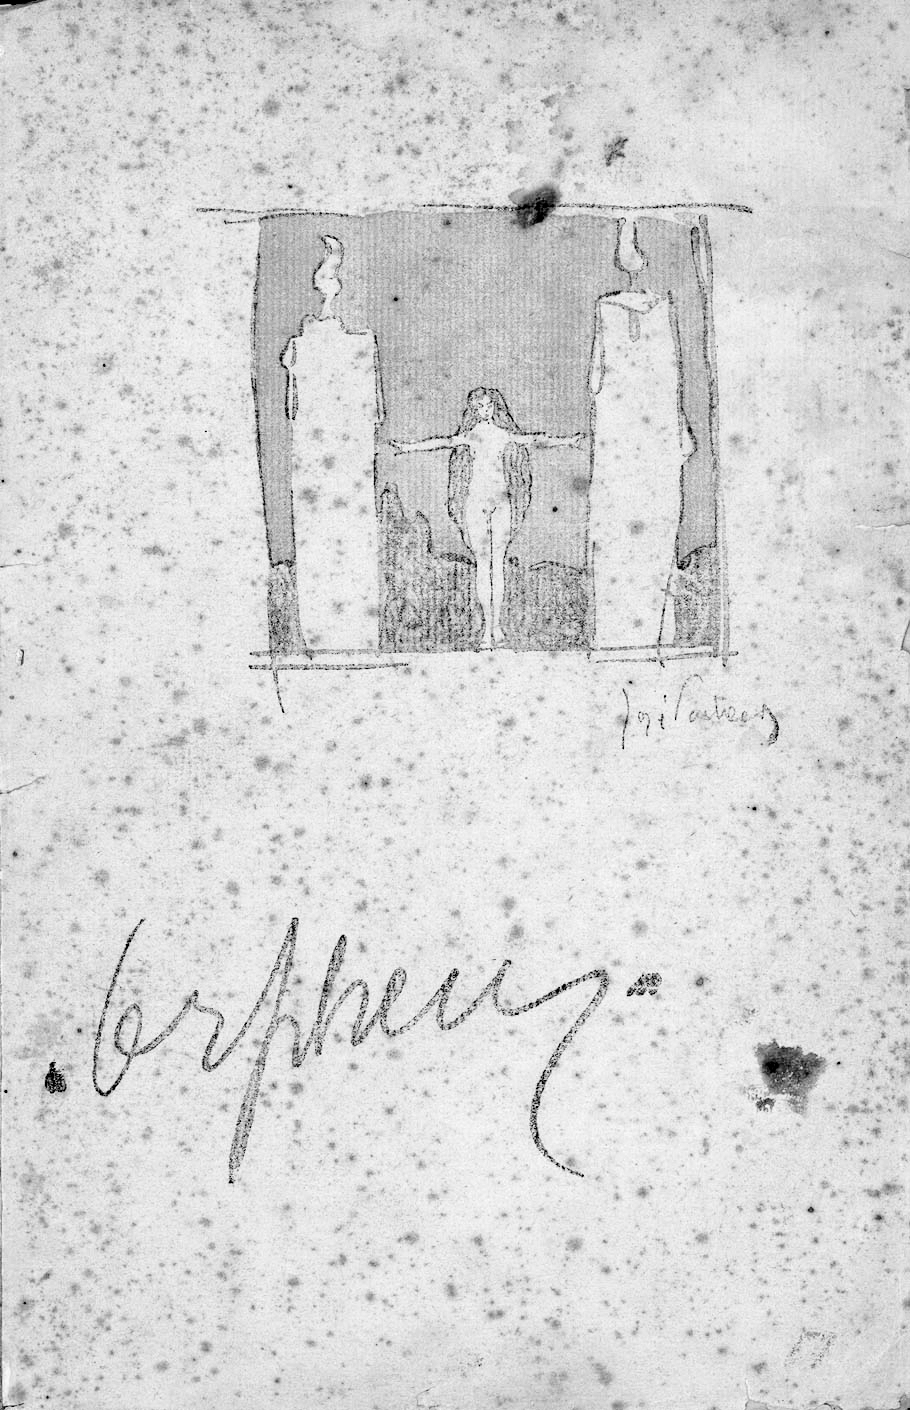
\includegraphics[width=\textwidth]{2.png}
\caption{Desenho reproduzido na capa da revista \emph{Orpheu}, n.~1.}
\end{figure}

Pessoa diz tê"-lo escrito na noite de 11
para 12 de setembro de 1913. Mas o texto 
foi publicado pela primeira vez dois anos
depois, na
\textit{Orpheu}, n. 1 (Lisboa, 1915).
A esse respeito, o autor observa ainda, 
numa carta enviada ao poeta e companheiro de geração Armando
Côrtes"-Rodrigues, que, entre a data da escrita e a
da publicação de seu
drama, submeteu"-o a uma profunda revisão,
deixando"-o bastante diferente
do que era em sua versão original; em suas palavras:

\begin{hedraquote}
O meu drama estático “O marinheiro” está bastante alterado e
aperfeiçoado; a forma que v. conhece é apenas a primeira e
rudimentar.
O final, especialmente, está muito melhor.
Não ficou, talvez, uma coisa
\textit{grande}, como eu entendo as coisas grandes;
mas não é coisa de
que me envergonhe, nem --- creio --- me
venha a envergonhar.\footnote{
Carta a Armando Côrtes"-Rodrigues, 4 de março de 1915.
\textit{In}: \textit{Fernando Pessoa ---
Correspondência 1905--1922}. Org.~de Manuela Parreira
da Silva. São Paulo: Companhia das Letras, 1999, p.~159.}
\end{hedraquote}

Aquilo que motivou tal revisão, e que é, portanto, determinante na
composição do texto de que dispomos, foi o fato de Álvaro Pinto,
diretor da revista \mbox{\textit{A águia}}, ter se recusado a publicar
\textit{O marinheiro}, em 1914, numa \textit{plaquette},
ou seja, num
pequeno folheto encadernado. Após esta rejeição 
e a decorrente revisão
do texto, a peça sairia não mais numa publicação de teor
saudosista,
mas no número de estreia da mais importante
revista modernista de seu
país, o que faz pensar no quão decisiva deve 
ter sido essa recusa na depuração da peça. 

A bem dizer, a recusa de Álvaro Pinto em publicar a peça numa
\textit{plaquette} do grupo da \textit{Renascença}
\textit{Portuguesa},
do qual \textit{A águia} era o órgão principal, 
foi o último episódio
relevante de um afastamento progressivo do
poeta com relação ao grupo
saudosista. A ruptura tardaria até o 
fim daquele ano para acontecer,
mas se observarmos com atenção, já o seu
texto anterior publicado na
revista, “Na floresta do alheamento”, 
sai com atraso de um número, o
que se documenta em carta de Pessoa
a seu editor nos seguintes termos:
“O ‘Na floresta do alheamento’ será ultraexcessivo, em matéria de
requinte, para que achem prudente que \textit{A águia} o insira?
Diga"-mo francamente.”\footnote{ Carta a Álvaro Pinto,
Lisboa, 29 de julho de 1913. \textit{In}: Fernando Pessoa --
\textit{Correspondência}
1905--1922. Op.~cit., 1999, p.~100.} 

Esse texto, que é um dos primeiros fragmentos do \textit{Livro do
desassossego}, naquele momento assinado 
com o próprio nome do poeta
(não existia, ainda, Bernardo Soares), apresenta uma atmosfera
decadente, tematiza o tédio e a inquietude existencial,
e representa
muito pouco o projeto \textit{renascente}.
Pessoa procurava desfiar, a
partir de uma sensação sua, a realidade interior, convertendo"-a,
através de imagens complexas, numa paisagem exterior.
Embora ainda com
ares decadentes, nesse momento se delineia pela obra de Pessoa uma
concepção que permanecerá muito sólida, e que o acompanhará até os
últimos poemas: “Quem quisesse resumir numa palavra a
característica
principal da arte moderna encontra"-la"-ia, 
perfeitamente, na palavra
\textit{sonho}. A arte moderna é arte de 
sonho.”\footnote{ O manuscrito
em que Pessoa faz essa afirmação é, segundo
os organizadores do volume,
provavelmente de 1913, o mesmo ano de escrita 
de \textit{O marinheiro}. Em
Fernando Pessoa. \textit{Páginas
de estética e de teoria e crítica
literárias}, op.~cit., p.~153.} 

Esse novo modo de encarar a arte,
que se afirma reiteradamente tanto na
prosa teórica de Pessoa quanto na do
\textit{Livro do desassossego}
(“Sonhar é encontrarmo"-nos. Vais ser o Colombo da
tua alma.”\footnote{ Bernardo Soares. 
\textit{Livro do desassossego}, org., intro. e notas
de Richard Zenith. São Paulo:
Companhia das Letras, 2006, p.~440.}),
despertava no próprio poeta a consciência
do quão distante ele já se
encontrava das diretrizes saudosistas.
Por esse motivo, quando Pessoa
antecipa a Álvaro Pinto o envio próximo de
\textit{O marinheiro}, já
tem, se observarmos com atenção, plena
consciência de que a peça não
poderia sair em \textit{A águia}: 

\begin{hedraquote}
Dentro em pouco, mandar"-lhe"-ei, para a \textit{Renascença}, caso queira
editar, um escrito meu --- uma peça em um ato, dum gênero especial a que
eu chamo \textit{estático}. Claro está que o meu amigo com toda a
franqueza me dirá, depois de ler a peça, se convém realmente editá"-la.
Exijo, e não me ofenderei com uma recusa --- uma franqueza absoluta.

A peça formará uma mera \textit{plaquette}. Não lha remeto para
\textit{A águia} porque para esse fim é, além de extensa, vagamente
imprópria.\footnote{ Carta a Álvaro Pinto,
Lisboa, 25 de maio de 1914.
Op.~cit., p.~116.}
\end{hedraquote}

Ao julgar que sua peça é imprópria para o órgão saudosista, Pessoa se
mostra ciente de que seu novo escrito anuncia caminhos inauditos não
apenas para o conjunto de sua obra, como para a literatura de seu país.
O que parece estar no gérmen dessa descoberta é a concepção de que a
tão obstinadamente perseguida “nova literatura” encerra a investigação
da própria alma do criador. É ainda em “Na floresta do alheamento” que
esse novo caminho vem anunciado, pouco depois
concretizado em \textit{O marinheiro}:

\begin{hedraquote}
O mais alto grau do sonho é quando, criado um quadro com personagens,
vivemos \textit{todas elas} ao mesmo tempo --- \textit{somos todas essas
almas conjunta e interativamente}. É incrível o grau de
despersonalização e encinzamento do espírito a que isto leva e é
difícil, confesso"-o, fugir a um cansaço geral de todo o ser ao
fazê"-lo\ldots{} Mas o triunfo é tal!\footnote{ Bernardo Soares. 
\textit{Livro do desassossego}. Op.~cit., p.~444.} 
\end{hedraquote}

Pessoa passaria então a levar às últimas consequências a concepção de
que a única realidade para si é ele próprio, e a investigar as leis de
sua personalidade através da tomada de consciência dos processos
mentais através dos quais se dão o conhecimento, as emoções e as
sensações, e, sobretudo, a refletir sobre como eles são convertidos em
arte. A literatura irá adquirir tal importância nesse processo, que
Pessoa assumirá que não sente, senão literariamente, que é poeta em
período integral, e que, portanto, o eu individual não está em lugar
algum: ele é muitos e nenhum ao mesmo tempo: 

\begin{hedraquote}
Tornei"-me uma figura de livro, uma vida lida. O que sinto é (sem que eu
queira) sentido para se escrever que se sentiu. O que penso está logo
em palavras, misturado com imagens que o desfazem, aberto em ritmos que
são outra coisa qualquer. De tanto recompor"-me destruí"-me. De tanto
pensar"-me, sou já meus pensamentos mas não eu. Sondei"-me e deixei cair
a sonda; vivo a pensar se sou fundo ou não, sem outra sonda agora senão
o olhar que me mostra, claro a negro no espelho do poço alto, meu
próprio rosto que me contempla contemplá"-lo.\footnote{ Ibid., p.~201.} 
\end{hedraquote}



\paragraph{Marinheiro -- Mensageiro}

Em \textit{O marinheiro}, as veladoras dizem não poder capturar o
presente --- em constante transição ---,
o passado --- que não é mais que um
sonho --- e o futuro --- que sumirá ao 
raiar do dia. Essa imaterialidade
aparentemente absurda só não resulta 
no \textit{nada} \textit{absoluto}
porque há a voz, único substrato de 
existência, o corpo irredutível do
drama (a \textit{palavra} --- as veladoras 
não são mais do que isso), que
paira numa atmosfera não exatamente onírica 
ou real, mas que se situa
no não"-espaço entre sonho e realidade:

\begin{hedraquote}
\repl{Primeira} [\ldots{}] Quando virá o dia?

\repl{Terceira} Que importa? Ele vem sempre
da mesma maneira\ldots{} sempre,
sempre, sempre\ldots{}

\hfill\paren{uma pausa}

\repl{Segunda} Contemos contos umas às
outras\ldots{} [\ldots{}] Neste momento eu não
tinha sonho nenhum, mas é"-me suave pensar
que o podia estar tendo\ldots{}
Mas o passado --- por que não falamos nós dele? 

\repl{Primeira} Decidimos não o fazer\ldots{} Breve raiará o dia e
arrepender"-nos"-emos\ldots{} Com a luz os sonhos adormecem\ldots{}
O passado não é
senão um sonho\ldots{} De resto, nem sei
o que não é sonho\ldots{} Se olho para o
presente com muita atenção, parece"-me que ele já passou\ldots{}
\end{hedraquote}


Por ser a voz o modo de existência no drama,
a segunda veladora, que por
vezes desempenha o papel de corifeu,
de narradora, conta seu sonho a
respeito de um marinheiro perdido numa
ilha longínqua. Impossibilitado
de voltar ao seu lugar de origem, ele, por
sua vez, sonha ter vivido
numa outra pátria, que constrói, dia a dia, pela imaginação. Aos
poucos, o marinheiro se torna capaz de enxergar
as paisagens, as ruas,
as cidades, pode percorrê"-las, 
reconhecer as pessoas que ali viveram,
seu passado e suas conversas, o lugar onde nasceu, onde passou as
diferentes fases da vida, e os companheiros
que teve. Mas eis que, num
dia de muita chuva, cansa"-se de sonhar, quer se lembrar da pátria
verdadeira, da meninice que teve, e então isso
lhe parece impossível,
nada lhe vem. Não pode nem ao menos 
supor ter vivido uma outra vida,
porque a única que teve passara a
ser realmente a vida que sonhara. 

A introdução do sonho do marinheiro na peça remonta à
origem da tragédia, que se baseia em antigas lendas 
que atravessavam os
séculos, perpetuando"-se pela tradição oral.
O sonho do marinheiro
carrega consigo uma espécie de aura mítica
em torno da criação, cujo
cerne reside na transposição do plano da imaginação para o da
realidade. Mais do que uma interpenetração de planos, 
trata"-se aqui de
se considerar o imaginário como
\textit{fundador} do real. Essa
concepção é fulcral para o “projeto 
civilizacional” que Pessoa traça em
sua obra: para ele, o Quinto Império 
português seria um “império de
poetas”, que se ergueria através do 
reconhecimento do valor de sua
língua, cuja forma de manifestação mais
elevada seria a sua poesia. A
função da heteronímia neste auspicioso plano 
seria a de dar a Portugal
os poetas que lhe faltavam. À parte o interesse
que esse projeto
desperta a respeito da megalomania de
seu criador, saliente"-se o seu
aspecto central: a fundação de uma
realidade, de uma pátria, pela
palavra. Não é a história que cria, 
são as lendas. O sonho do
marinheiro pode nos remeter, por exemplo,
à lenda popular segundo a
qual Lisboa teria sido fundada pelo herói grego Ulisses (outro
marinheiro). “Olissipona” seria já a corruptela de Olissipo, que
significa “a cidade de Ulisses”.
O próprio Pessoa registra no aforismo de abertura
de um de seus poemas mais célebres, ``Ulisses'', a refundição da 
realidade pelo mito: ``O mito é o nada que é tudo”. O
livro em que este poema se encontra,
\textit{Mensagem} (marco final, e
portanto diametralmente oposto a 
\textit{O marinheiro}, do percurso poético pessoano) é, por
sua vez, a construção de um mito a entrar
pela realidade, a exemplo do
sebastianismo, que o atravessa do começo ao fim. 

O que é mais real? Qual é o estatuto da realidade?
Ainda no poema “Ulisses”, lê"-se: 
\begin{hedraquote}
\begin{verse}
Este que aqui aportou\\
Foi por não ser existindo\\ 
Sem existir nos bastou.
\end{verse}
\end{hedraquote}
Uma vez incorporada ao
folclore, a lenda se torna realidade. 
O sonho do marinheiro representa,
portanto, um papel"-chave na peça, ao se revelar 
análogo à mais larga
utopia de seu autor. A pátria de sonho 
substitui na peça a pátria real: “Todo este
país é muito triste\ldots{}”, afirma a segunda veladora. Ora, se
o marinheiro sonha com uma pátria oposta à
real, referida pela veladora
com a expressão “este país”, o que de
fato ela vela senão “este país”?
A morta não será já a pátria portuguesa? 

A fala da segunda veladora prossegue: “Aquele (país) onde eu vivi
outrora era menos triste”. Esse “outrora” apresenta uma densidade
específica na poesia de Pessoa.
Trata"-se de um passado onírico, isto é,
um produto presente da imaginação, algo que foi sem nunca ter
sido. O passado em Pessoa é uma de suas principais
máscaras; traz, em síntese, esse revestimento de realidade vivida,
sobre um miolo que se compõe da mesma matéria dispersa do sonho. 


Álvaro de Campos, outro “marinheiro” célebre
de Pessoa --- mas, notemos
bem, um marinheiro em sonho, que na sua fase mais estridente, da
colossal “Ode marítima”, singra os oceanos sem
realmente sair do cais ---
também constrói sua utopia num espaço"-tempo 
arquetípico, resgatado de
um ideal “outrora”:

\begin{hedraquote}
\begin{verse}
Ah, quem sabe, quem sabe,\\
Se não parti \textit{outrora}, antes de mim,\\
Dum cais; se não deixei, navio ao sol\\
Oblíquo da madrugada,\\
Uma outra espécie de porto?\\
Quem sabe se não deixei, antes da hora\\
Do mundo exterior como eu o vejo\\
Raiar"-se para mim,\\
Um grande cais cheio de pouca gente,\\
Duma grande cidade meio"-desperta,\\
Duma enorme cidade comercial, crescida, \qb apopléctica,\\
Tanto quanto isso pode ser fora do Espaço e \qb do Tempo?\footnote{ 
Álvaro de Campos. “Ode marítima”, \textit{in}:
 \textit{Obra poética}. Rio de Janeiro:
Nova Aguilar,
1966, pp.~315--16. O grifo é nosso.}
\end{verse}
\end{hedraquote}

Na “Ode marítima”, a exemplo do que ocorre em
\textit{O marinheiro}, o
sonho de um porto infinito, de um cais
absoluto, sempre projetado para
um passado primordial, “antes da hora”, se delineia através de
calafrios e arroubos da consciência de Campos, de modo similar aos
rompantes das veladoras, que a todo momento
questionam o estatuto da
própria fala. Esse sonho do marinheiro,
de uma ilha “longínqua”, remete
já à “Distância Absoluta”, ao “Puro Longe,
liberto do peso do Atual”,
que confere densidade arquetípica ao poema de Campos. Em ambos os
textos, há uma voz absoluta que atua sobre
seus protagonistas como o
canto das sereias, o chamamento das águas:
em Campos, o grito surdo e
gutural do marinheiro Jim Barns; na peça, o próprio sonho do
marinheiro, que hipnotiza as veladoras. O eu lírico
Álvaro de Campos sonha"-se marinheiro, e
para ele, como para Pessoa, a
segunda veladora parece apontar
quando afirma sobre o marinheiro da
peça: “Toda a sua vida tinha sido a sua vida que sonhara\ldots{}”.
Analogamente, no poema lemos: 
“A minha alma está com o que vejo menos”.
Essa ânsia comum pelo ancestral 
confere aos textos o sentido mais vasto
de uma expedição psíquica. De resto, 
o universo marítimo, tanto na peça
quanto no poema, recompõe leituras da infância de Pessoa, como de
\textit{A ilha do tesouro}, de Robert Louis Stevenson.


Essas considerações se devem ao alto grau
de conotação que o advérbio
“outrora” desempenha na peça,
cujo papel é, em síntese, o de compor
fora do eu sua vida interior.
Essa leitura não suplanta, contudo, uma
importante referência histórica que,
aproximada ao corpo do texto,
mostra"-se especialmente relevante. 

O país em que a veladora diz ter vivido “outrora” é
já, provavelmente, um Portugal anterior à profunda
crise política que
marca a infância de Pessoa em Lisboa.
Na última década do século \textsc{xix},
Portugal passa por uma de suas maiores
humilhações internacionais, o
\textit{Ultimatum} inglês, de 1890.
A Inglaterra exige, sob pena de
invadir o país, que o rei retire suas tropas 
da região do Xire, na
África, o que acarreta, com fortes ecos 
culturais, uma grave crise de
identidade e orgulho próprio em sua população.
Analogamente, a volta de
Pessoa à terra natal, após receber durante nove anos uma formação
tradicionalmente inglesa, em Durban, 
na África do Sul, situa"-se pouco
antes do regicídio de 1908, isto é, 
do brutal assassinato do rei D.~Carlos
e do príncipe herdeiro por um fanático republicano, e pela
decorrente proclamação da República, em 1910. 

Além disso, vale a pena considerar que
entre os episódios de 1890 e
1910, a infância e juventude do poeta estão longe de ser o éden, o
“outrora” projetado em seus poemas 
(Pessoa diz sentir saudade da
``criança feliz que nunca fui”). A passagem por
esse período, a bem dizer
um calvário familiar, deixa"-lhe profundas
cicatrizes, causadas por uma
sequência trágica de acontecimentos, ocorridos
até seus treze anos: a
morte do pai, Joaquim de Seabra Pessoa, 
a mudança de casa, com a maior
parte de seus bens tendo sido leiloados,
a morte de seu irmão, Jorge, a
morte da avó materna, a internação da outra avó, Dionísia, sob o
diagnóstico de demência, devido às suas atividades mediúnicas, 
a despedida da
terra natal e a morte da irmã, Madalena, 
antes de completar três anos.


Esses elementos históricos e biográficos não explicam,
evidentemente, a peça. Apenas podem ser
indiretamente referidos a ela.
Sua internalização em \textit{O
marinheiro}, particularmente na passagem “Todo esse
país é muito triste\ldots{}”, associada ao registro
que lhe é próprio
(segundo o qual as personagens não
são nomeadas ou caracterizadas),
conduz a uma abertura de sentidos.
Dessa perspectiva, a donzela morta,
mistério mudo, corpo velado até o raiar de uma nova manhã (de uma
\textit{renascença}, portanto),
apresenta notável analogia com o cadáver de 
Portugal, especificamente a
pátria da infância de Pessoa. 

Essa leitura da peça, que a situa, no itinerário
poético de Pessoa, como linha de partida de
\textit{Mensagem}, confirma"-se no
seu desfecho, em que a terceira
veladora, com uma voz “muito lenta e
apagada”, anuncia: “Ah, é agora, é
agora\ldots{} Sim, acordou alguém\ldots{} Há
gente que acorda\ldots{} Quando 
entrar alguém tudo isto acabará\ldots{}”. 

O arremate em tom de anúncio é analogamente marcante em
\textit{Mensagem}. Em seu poema final, “Nevoeiro”,
que identifica a
atmosfera dispersa e brumosa da peça,
a imagem de um país em decadência
é claramente retomada: 
\begin{hedraquote}
\begin{verse}
Ninguém sabe que coisa quer.\\
Ninguém conhece que alma tem,\\
Nem o que é mal nem o que é bem.\footnote{  Fernando Pessoa.
\textit{Mensagem}. Org., intro.,
posf.~e glossário de Caio
Gagliardi. São Paulo: Hedra, 2007, p.~118.}
\end{verse}
\end{hedraquote}


É significativo considerar que entre 
1910 e 1928, a data de escrita
desse poema, a sociedade portuguesa
passou por uma profunda crise de
valores diante do forte clima de revanchismo e turbulência
político"-social. Após o já referido
assassinato do rei D.~Carlos e do
príncipe herdeiro D.~Felipe, o assassinato
do presidente Sidónio Pais,
em 1918, e o golpe militar de 1926 tornam ainda mais aguda a crise
nacional. Em “Nevoeiro” lê"-se:\EP[1]
\begin{hedraquote}
\begin{verse}
Nem rei nem lei, nem paz nem guerra,\\
Define com perfil e ser\\ 
Este fulgor baço da terra\\ 
Que é Portugal a entristecer.\footnote{ Ibid., p.~118.}
\end{verse}
\end{hedraquote}

O mesmo triste país referido
pela segunda veladora em \textit{O marinheiro} é aqui retomado. 

Na peça, o raiar do dia substitui o Portugal do “hoje és
Nevoeiro”\footnote{ Ibid., p.~118.} pelo Portugal do “poder
ser”.\footnote{ “Tormenta”, em 
\textit{Mensagem}, op.~cit, p.~115.} A
intuição da veladora, “Ah, é agora, 
é agora\ldots{}”, continua a ser ouvida
em \textit{Mensagem}, como uma paronomásia
lançada a \textit{O
marinheiro}, no seu verso mais profético e,
muito significativamente,
derradeiro: “É a hora!”. Não acidentalmente,
a chegada desse “novo dia”
põe fim ao velório e arremata a peça.
O tempo arquetípico de \textit{O
marinheiro} é o da “Antemanhã”,
título de um poema da parte final de
\textit{Mensagem}, tempo do prenúncio, da “madrugada do novo dia”. 

\textit{O marinheiro} (1915)
e \textit{Mensagem} (1934) identificam
as duas pontas da linha utópica que se
desenrola pelo percurso poético pessoano.

\paragraph{A quinta pessoa}

O dia começa a raiar e tanto a ilha
do marinheiro quanto o quarto com as
veladoras parecem"-lhes igualmente
irreais. Não será tudo sonho? Pela
fala da segunda veladora: “Talvez
nada disto seja verdade\ldots{} Todo este
silêncio e esta morta, e este dia que
começa não são talvez senão um
sonho\ldots{} Olhai bem para tudo
isto\ldots{} Parece"-vos que pertence à
vida?\ldots{}”. E então o caráter
ficcional do sonho narrado se inverte. O
pavor criado pela hipótese de não existirem, 
de tudo não passar de
poeira dos sonhos, recai sobre as
veladoras: “Por que não será a única
coisa real nisto tudo o marinheiro,
e nós e tudo isto aqui apenas um
sonho dele?”. Eis um dos momentos"-chave
para se compreender a peça. 

Na medida em que o que garante a 
permanência das veladoras no mundo é a
fala, estranhar a própria voz significa
questionar a existência. Esse
questionamento ganha consistência no
drama com horror crescente, como
se houvesse uma mão oculta, uma “quinta pessoa”
(além das três donzelas
e do corpo velado) guiando suas falas. 
São muitos os trechos que
alimentam esse estranhamento: 
“Entre mim e a minha voz abriu"-se um
abismo”; “Agora estranho"-me viva com
mais horror”; “E parecia"-me que
vós, e a vossa voz, e o sentido do que 
dizíeis eram três entes
diferentes, como três criaturas que
falam e andam”; “Dói"-me o intervalo
que há entre o que pensais e o que
dizei\ldots{} A minha consciência boia à
tona da sonolência apavorada dos meus 
sentidos pela minha pele\ldots{}”;
“Oh, que horror, que horror íntimo nos desata a voz da alma, e as
sensações dos pensamentos, e nos
faz falar e sentir e pensar quando
tudo em nós pede o silêncio e o dia
e a inconsciência da vida\ldots{}”. 

É com esse arrepio da consciência que tocamos 
o cerne da peça --- e
porventura da obra de Pessoa ---, assim 
identificado, em outro contexto,
por José Augusto Seabra: “a desintegração
da linguagem numa pluralidade
de linguagens (o poemodrama), do sujeito
numa pluralidade de sujeitos
(o poetodrama)”.\footnote{ 
José Augusto Seabra. \textit{Fernando Pessoa
ou o poetodrama}. Op.~cit., p.~31.} 

Pessoa traça aqui o processo de desprendimento do eu de si mesmo, como
uma consciência boiando sobre a sensação, e das sensações sentindo,
portanto, a sós, apostasiadas, isto é, desvinculadas de uma mente e de
um corpo. Em retrospectiva, o desdobramento heteronímico parece
prefigurado. Em \textit{O marinheiro} esse desdobramento traduz"-se
abertamente como reflexão profunda a respeito de um tema que é
obsessivamente perseguido nas diferentes instâncias da obra: o mistério
do ser. De modo similar, o paradoxo da escrita reside na
impossibilidade de se fixar uma unidade existencial: quando o escritor
diz “eu”, quem é o eu que fala? Essa clivagem, que é própria da
enunciação, é obsessivamente retomada na peça.

Uma das leituras mais radicais deste drama (embora muito breve) é
realizada pelo escritor italiano Antonio Tabucchi, que se afasta da
habitual aproximação feita pela crítica com os dramas simbolistas, e
entende \textit{O marinheiro} como uma charada shakespeariana que exibe
o centro dramático,\footnote{ Antonio Tabucchi. \textit{Pessoana
mínima}: escritos sobre Fernando Pessoa. Lisboa: Imprensa Nacional --
Casa da Moeda, 1984.} ou, se preferirmos, a metalepse (a transposição
de planos ficcionais) da escrita pessoana: o problema de se traduzir
uma ficção por outra ficção --- a vida, que não passa de um sonho, pela
literatura, o teatro. 

Tabucchi não desenvolve essa leitura, mas se pode considerar que toda a
obra de Pessoa é vazada por essa voz em surdina, esse coro da
consciência refletindo os passos de seus protagonistas. Nesse sentido,
estaremos diante de um texto de alcance metalinguístico, no qual,
possivelmente, a \textit{quinta pessoa} pressentida no quarto (“Quem é
a quinta pessoa neste quarto que estende o braço e nos interrompe
sempre que vamos a sentir?”) é o próprio autor --- lembrando, é claro,
que o autor no texto é sempre uma
\textit{persona}, uma criação. O
tônus poético que Pessoa já manifesta em sua peça não é de natureza
diversa ao do drama grego, a dizer, a interação crítica entre o coro,
mantenedor da voz da razão, e a personagem. O primeiro, a observar e
interpretar a ação, atua como uma consciência intromissiva sobre a
sensação, como se ele fosse um espectador ideal do próprio drama. 

Em \textit{O marinheiro}, não estarão as veladoras prestes a romper a
bolha que as separa do mundo não"-ficcional? Não serão elas, a exemplo do
espetacular drama heteronímico, personagens em busca de um autor? Isto
é, em busca daquele que as conduz, que dita suas vozes. “Quem é que nos
faz continuar falando?”, indaga uma delas. E a consciência da outra lhe
insufla de uma vida que parece já não ser a de seu autor: “Que estranha
que me sinto!\ldots{} Parece"-me já não ter a minha voz\ldots{} Parte de mim
adormeceu e ficou a ver\ldots{}”. Não estaremos, neste ponto exato, na
iminência de desatar o nó górdio da representação: a transformação de
uma personagem em autor? 

Personagens, portanto, em quem a busca por um autor conduz a uma
condição mais especial: a do encontro com a própria autoria, do autor
em si --- autor de si.

A aproximação do drama a \textit{Seis personagens à procura de um
autor}, de Pirandello, é profícua a essa leitura. À pergunta “Quem é
que nos faz continuar falando?”, Pirandello parece fornecer
inequívoca resposta.

O marinheiro, que é “sonho de um sonho” --- que é
fruto da imaginação da segunda veladora, que, por sua vez, é fruto da
imaginação do poeta ---, quando começa a sonhar, produz uma nova
realidade, uma terceira dimensão, portanto, que é seu próprio passado.
Acrescente"-se a esse tema, aqui já tratado, que essa construção do passado, que só passa a existir no momento da
lembrança (uma lembrança imaginária, portanto), Pessoa condensou com o
brilho característico na expressão “outrora agora”, no poema “Pobre
velha música!”.\footnote{ Fernando Pessoa. \textit{Obra poética}. Op.~cit.,
p.~141.} Também em “Lisbon revisited (1923)”\footnote{ 
Álvaro de Campos. \textit{Obra poética}. Op.~cit., p.~357.} lemos “Lisboa de
outrora de hoje”. Em \textit{O marinheiro}, cerca de uma
década antes da escrita desses poemas, à pergunta da segunda veladora,
“Éreis feliz, minha irmã?”, a primeira responde: “Começo neste momento
a tê"-lo sido outrora\ldots{}”. Na poesia de Pessoa, conforme antecipado na
fala da primeira veladora, “O passado não é senão um sonho\ldots{} De resto,
nem sei o que não é sonho”.

Essa mudança de estatuto do real na peça, de um passado que nunca
existiu, porque apenas se torna realidade quando é lembrado no
presente, decorre, em síntese, da seguinte metamorfose: o marinheiro,
de sonhado torna"-se sonhador; de personagem migra para o lado do autor.


Enunciador similar ao marinheiro pode ser
identificado em
\textit{Mensagem}, no poema “As
ilhas afortunadas”: 
\begin{hedraquote}
\begin{verse}
Que voz vem no som das ondas\\
Que não é a voz do mar?\\ 
É a voz de alguém que nos fala,\\
Mas que, se escutamos, cala,\\
Por ter havido escutar.
\end{verse}
\end{hedraquote}

É agora o marinheiro, produto do sonho, quem narra. Feito isso, Pessoa
inverte papéis e polos referenciais: a aparência ilusória de verdade, a
“verdade fingida” que se encontra no plano das veladoras, torna"-se
menos real do que aquilo que o marinheiro sonhou (do sonho --- do
marinheiro --- dentro do sonho --- da segunda veladora --- dentro do sonho ---
do próprio autor). Assim, a pátria sonhada torna"-se uma ficção mais
verdadeira do que a anterior. 

A feliz e, de certo, insuperável síntese desse imbricamento mútuo,
Pessoa nos legou ainda muito cedo, em um trecho do seu “Na floresta do 
alheamento”: “E assim nós morremos a
nossa vida, tão atentos separadamente a morrê"-la que não reparamos que
éramos um só, que cada um de nós era uma ilusão do outro, e cada um,
dentro de si, o mero eco do seu próprio ser\ldots{}”.\footnote{ 
Bernardo Soares. \textit{Livro do desassossego}. Op.~cit., p.~457.}

A vida é sonho. E este problema tão pessoano está, afinal, e segundo
Tabucchi, já explícito no teatro de Shakespeare. Quando Pessoa declara
``\textit{All my books are books of reference. I read Shakespeare only in
relation to the} Shakespeare Problem: \textit{the rest I know
already}'',\footnote{ Fernando Pessoa. \textit{Páginas íntimas de
autointerpretação}. Op.~cit, pp.~20--1. Apud. Tabucchi, Antonio. Op.
cit., p.~88.} faz menção a um problema que é tanto seu quanto do autor
inglês --- e, de resto, de toda a literatura. 

Claro está, portanto, que \textit{O marinheiro} apresenta, ainda que de
modo velado, uma forte reflexividade discursiva, que se manifesta tanto
no nível do enunciado (nos momentos em que as personagens se
questionam) como no nível da enunciação (nos momentos em que essas
vozes se confundem com uma instância elocutória exterior à estrutura da
peça, isto é, a voz autoral). Ler (mas sobretudo reler)
\textit{O marinheiro} consiste, assim, na engenhosa tarefa de se
descobrir véus por trás de véus, caixas dentro de caixas (a exemplo das
\textit{matrioskas}, as bonecas
russas feitas de madeira oca, que englobam umas às outras), teatros
espelhando teatros. Lê"-lo é já, portanto, cair num abismo (\textit{mise
en abyme}) existencial, do qual transborda a consciência absolutamente
ativa e lúdica de seu autor.  

Em \textit{O
marinheiro}, o teatro assume o estatuto de metáfora
mais ampla do jogo ilusório a que se destina o conhecimento de
categorias outrora transparentes, tornadas instáveis na modernidade: o
\textit{autor} e a
\textit{personagem}, a
\textit{identidade} e a
\textit{alteridade}, a
\textit{ficção} e a
\textit{realidade}. Aqui, esses
pares aparecem não apenas indistintos, como trocados. 

No conjunto da obra de Pessoa, \textit{O marinheiro} 
é uma primeira
tentativa de traduzir, no plano do teatro, o teatro da vida. 

Talvez não seja mero acaso que no ano seguinte à sua escrita esse drama
notável tivesse sido sucedido por outro ainda mais vertiginoso, o da
heteronímia.

\section{Nota à edição}

Os textos aqui publicados, além de revisados, foram adaptados para o
português falado no Brasil, o que não alterou o texto original, a não
ser pela supressão do efeito de estranhamento que alguns empregos
específicos poderiam provocar. Entre as adaptações realizadas
estão a substituição de “cousa” por “coisa”, a exclusão do “c” mudo em
casos como “abstracto”, a eliminação do hífen em casos como “há-de”, a
supressão ou a substituição do acento agudo em ocorrências como
“amámos” e “prémio”, a eliminação do pronome em “até ao” (pouco usado
no Brasil, mas padronizado em Portugal), e a substituição de “de mais”
por “demais”, quando advérbio. Sempre que a ocorrência resultou em
efeito expressivo, tal como o uso da letra minúscula sucedendo o ponto
final, o emprego do hífen em casos como “pela porta todas-as-portas”, e
a inexistência de vírgula antes da adversativa “mas”, manteve-se a
escrita original. 

A ordenação dos textos, por sua vez, não obedece a
um critério cronológico, dada a impossibilidade de o fazer, tampouco a
algum outro critério rígido, por não se tratar aqui de uma
\textit{edição crítica}. Os trechos em que a transcrição foi impossível
ou duvidosa estão marcados, respectivamente, por [\ldots] e [?], e 
a opção por colocar o restante do nome dos personagens entre colchetes 
quando no original só aparecia a primeira letra (como, por exemplo, S[alomé])
foi do primeiro editor e aqui mantida. Optamos,
ainda, por incluir no final das peças os fragmentos soltos, referentes
ao diálogo, mas sem arrumação do autor. 



\begin{bibliohedra}

\tit{Balakian}, Anna. \textit{O simbolismo}, São Paulo,
Perspectiva, 1985.

\tit{Bréchon}, Robert. \textit{Estranho estrangeiro},
Rio de Janeiro, Record, 2000.

\tit{Horácio}, \textit{Arte poética}. Ed.~Bilíngue. 
Trad.~de R.~M.~Rosado Fernandes. Lisboa: Clássica, s.d.

\tit{Lopes}, Teresa Rita. \textit{Fernando Pessoa et le drame simboliste: héritage et création.}
2\oi ed. Foundation Calouste Gulbenkian: Centre Cultural Portugais, 1985.

\tit{Pessoa}, Fernando. \textit{Correspondência}
1905--1922. Org.~de Manuela Parreira da Silva. São Paulo:
Companhia das Letras, 1999. 

\tit{\_\_\_\_\_\_}. \textit{Mensagem}, org., intro., posf.
e glossário por Caio Gagliardi. São Paulo, Hedra, 2007.

\tit{\_\_\_\_\_\_}. \textit{Obra poética}, 
Rio de Janeiro,
Nova Aguilar, 1966.

\tit{\_\_\_\_\_\_}. \textit{Páginas de estética e de teoria e
crítica literárias}, 2ª. ed., org.~de Georg Rudolf Lind e Jacinto do
Prado Coelho, Lisboa, Ática, 1973.

\tit{Seabra}, José Augusto. \textit{Fernando Pessoa ou o
poetodrama}, São Paulo, Perspectiva, 1974.

\tit{Sêneca}, \textit{Agamêmnon}, trad., intro., posf.~e notas
por José Eduardo Lohner, São Paulo, Globo, 2009.

\tit{Soares}, Bernardo. \textit{Livro do desassossego}, org.,
intro.~e notas por Richard Zenith, São Paulo, Companhia das Letras,
2006.

\tit{Tabucchi}, Antonio. \textit{Pessoana mínima}: escritos
sobre Fernando Pessoa, Lisboa, Imprensa Nacional -- Casa da Moeda,
1984.
\end{bibliohedra}
